\documentclass[aspectratio=169]{beamer}
\usepackage[utf8]{inputenc}
\usepackage{amsmath}
\usepackage{tikz}
\usepackage{dsfont}
\usepackage{opensans}
\usepackage{xcolor}

\newtheorem{proposition}{Proposition}

\title[]{4509 - Bridging Mathematics}
\subtitle{Concavity and Quasiconcavity}
\author[P. Fagandini]{Paulo Fagandini}
\institute[]{}
\date{}

\usetheme{NOVASBE}

\begin{document}

\begin{frame}{Concavity}

\begin{definition}[Concave and Convex function]
    A real-valued function $f:\mathcal{U}\subseteq \mathbb{R}^n$ is \textbf{concave} if $\forall x,y \in\mathcal{U}$ and $\forall t\in[0,1]$:
    \[f(tx+(1-t)y)\geq tf(x)+(1-t)f(y)\]
    and it is \textbf{convex} if
    \[f(tx+(1-t)y)\leq tf(x)+(1-t)f(y)\]
\end{definition}

\end{frame}

\begin{frame}{Concavity}
    Concavity and convexity of a function have also a geometric interpretation.    
    \vspace{1em}

    \begin{proposition}
        A function $f:\mathcal{U}\subseteq \mathbb{R}^n\rightarrow\mathbb{R}^m$ is concave (convex) $\Leftrightarrow$ $\forall x,y\in\mathbb{R}^n$ the secant line connecting $x$ and $y$ lies \textit{below (above)} the graph of $f$.
    \end{proposition}

\end{frame}

\begin{frame}{Concavity}
    \begin{center}
        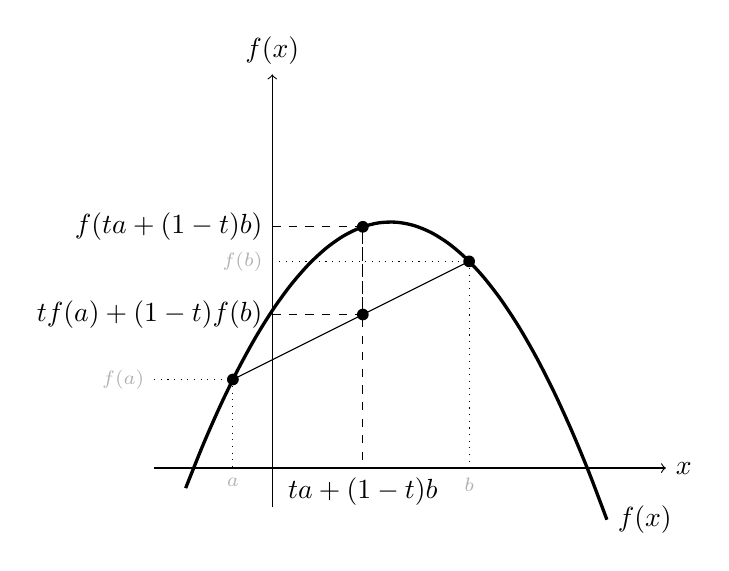
\begin{tikzpicture}[declare function = {
                f(\x)=-0.5*(\x+1)*(\x-4);
                }]

            \def\a{-0.5}
            \def\b{2.5}
            \def\t{0.45}

            \draw[->] (-1.5,0) -- (5,0)node[right]{$x$};
            \draw[->] (0,-0.5) -- (0,5)node[above]{$f(x)$};

            \draw (\a,{f(\a)})node[circle,fill,inner sep= 1.5pt]{} -- (\b,{f(\b)})node[circle,fill,inner sep= 1.5pt]{};

            \draw[dotted] ({\a-1},{f(\a)})node[left, color=black!30]{\scriptsize{$f(a)$}} -- (\a,{f(\a)});
            \draw[dotted] (0,{f(\b)})node[left, color=black!30]{\scriptsize{$f(b)$}} -- (\b,{f(\b)});

            \draw[dotted] (\a,{f(\a)}) -- (\a,0)node[below, color=black!30]{\scriptsize{$a$}};
            \draw[dotted] (\b,{f(\b)}) -- (\b,0)node[below, color=black!30]{\scriptsize{$b$}};

            \draw[dashed] (0,{f(\t*\a+(1-\t)*\b)}) node[left]{$f(ta+(1-t)b)$} -- 
                ({\t*\a+(1-\t)*\b},{f(\t*\a+(1-\t)*\b)})node[circle,fill,inner sep= 1.5pt]{} -- 
                ({\t*\a+(1-\t)*\b},0)node[below]{$ta+(1-t)b$};

            \draw[dashed] (0,{\t*f(\a)+(1-\t)*f(\b)})node[left]{$tf(a)+(1-t)f(b)$} --
                ({\t*\a+(1-\t)*\b},{\t*f(\a)+(1-\t)*f(\b)})node[circle,fill,inner sep=1.5pt]{} --
                ({\t*\a+(1-\t)*\b},{f(\t*\a+(1-\t)*\b)});

            \draw[domain=-1.1:4.25, very thick, smooth] plot (\x,{f(\x)})node[right]{$f(x)$};
        \end{tikzpicture}
    \end{center}
    
\end{frame}

\begin{frame}{Convexity}
    \begin{center}
        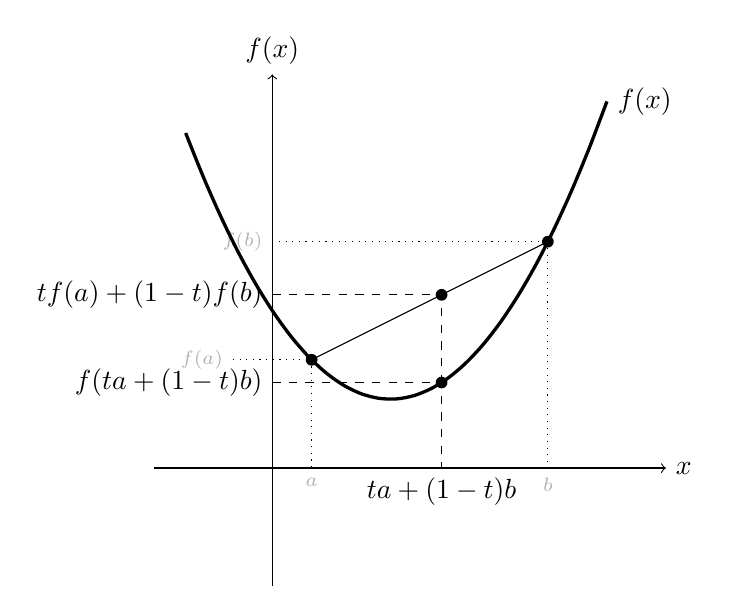
\begin{tikzpicture}[declare function = {
                f(\x)=0.5*(\x+1)*(\x-4)+4;
                }]

            \def\a{0.5}
            \def\b{3.5}
            \def\t{0.45}

            \draw[->] (-1.5,0) -- (5,0)node[right]{$x$};
            \draw[->] (0,-1.5) -- (0,5)node[above]{$f(x)$};

            \draw (\a,{f(\a)})node[circle,fill,inner sep= 1.5pt]{} -- (\b,{f(\b)})node[circle,fill,inner sep= 1.5pt]{};

            \draw[dotted] ({\a-1},{f(\a)})node[left, color=black!30]{\scriptsize{$f(a)$}} -- (\a,{f(\a)});
            \draw[dotted] (0,{f(\b)})node[left, color=black!30]{\scriptsize{$f(b)$}} -- (\b,{f(\b)});

            \draw[dotted] (\a,{f(\a)}) -- (\a,0)node[below, color=black!30]{\scriptsize{$a$}};
            \draw[dotted] (\b,{f(\b)}) -- (\b,0)node[below, color=black!30]{\scriptsize{$b$}};

            \draw[dashed] (0,{f(\t*\a+(1-\t)*\b)}) node[left]{$f(ta+(1-t)b)$} -- 
                ({\t*\a+(1-\t)*\b},{f(\t*\a+(1-\t)*\b)})node[circle,fill,inner sep= 1.5pt]{} -- 
                ({\t*\a+(1-\t)*\b},0)node[below]{$ta+(1-t)b$};

            \draw[dashed] (0,{\t*f(\a)+(1-\t)*f(\b)})node[left]{$tf(a)+(1-t)f(b)$} --
                ({\t*\a+(1-\t)*\b},{\t*f(\a)+(1-\t)*f(\b)})node[circle,fill,inner sep=1.5pt]{} --
                ({\t*\a+(1-\t)*\b},{f(\t*\a+(1-\t)*\b)});

            \draw[domain=-1.1:4.25, very thick, smooth] plot (\x,{f(\x)})node[right]{$f(x)$};
        \end{tikzpicture}
    \end{center}
    
\end{frame}

\begin{frame}{Concavity}
    \begin{definition}[Convex Set]
    A set $\mathcal{U}$ is said to be \emph{convex} if $\forall x,y\in\mathcal{U}$ and $\forall t\in[0,1]$ it holds that:
    \[tx+(1-t)y \in \mathcal{U}\]
    \end{definition}
    
    \underline{Facts:}
    \begin{enumerate}
        \item It is not uncommon to call $tx+(1-t)y$ with $t\in[0,1]$ a \textit{convex combination} between $x$ and $y$.
        \item A \textcolor{red}{\textbf{concave set}}, contrary to functions, is \textcolor{red}{\textbf{not a thing}}.
    \end{enumerate}
\end{frame}

\begin{frame}{Concavity}
    \begin{proposition}
        All convex or concave functions must have a \textit{convex} domain.
    \end{proposition}

    \begin{proposition}
        \begin{enumerate}
            \item $f$ is concave if and only if the set below its graph $\{(x,y) : y \leq f(x)\}$ is convex.
            \item $f$ is convex if and only if the set above its graph $\{(x,y): y \geq f(x)\}$ is convex.
        \end{enumerate}    
    \end{proposition}
\end{frame}

\begin{frame}{Concavity}
    \begin{theorem}
        Let $f:\mathcal{U}\subseteq\mathbb{R}^n\rightarrow\mathbb{R}^n$. Then, $f$ is concave (convex) if and only if its restriction to every line segment in $\mathcal{U}$ is a concave (convex) function of one variable.
    \end{theorem}
\end{frame}

\begin{frame}{Concavity}
    \begin{proof}
        \(\Leftarrow\)

        Let $x,y\in\mathcal{U}$ and $g(t)=f(tx+(1-t)y)$. By hypothesis, $g$ is concave.
        \begin{align*}
            f(tx+(1-t)y)&=g(t)\\
            &=g(t\times 1+(1-t)\times 0)\\
            &\geq t g(1)+(1-t)g(0)\\
            &= tf(x)+(1-t)f(y)
        \end{align*}
        And then $f$ is concave.
    \end{proof}
\end{frame}

\begin{frame}{Concavity}
    \begin{proof}
        \(\Rightarrow\)
        
        Let $s_1$ and $s_2$ in the domain of $g$. Let $t\in[0,1]$.
        \begin{align*}
            g(ts_1+(1-t)s_2)&=f((ts_1+(1-t)s_2)x+(1-(ts_1+(1-t)s_2))y)\\
            &= f(t(s_1x+(1-s_1)y)+(1-t)(s_2x+(1-s_2)y))\\
            &\geq tf(s_1x+(1-s_1)y) + (1-t)f(s_2x+(1-s_2)y)\\
            &=tg(s1)+(1-t)g(s_2)
        \end{align*}
        And then $g$ is concave.
    \end{proof}
\end{frame}

\begin{frame}{Concavity}
    \begin{theorem}
        Let $f$ be a $C^1$ function on an interval $I\subset \mathbb{R}$. Then, $f$ is concave on $I$ if and only if:
        \[f(y)-f(x)\leq f'(x)(y-x),\ \forall x,y\in I\]
        $f$ is convex if:
        \[f(y)-f(x)\geq f'(x)(y-x),\ \forall x,y\in I\]
    \end{theorem}
    
\end{frame}

\begin{frame}{Concavity}
    \begin{proof}
        \(\Rightarrow\)

        Let $f$ be a concave function on $I$, $x,y\in I$ with $x\neq y$, and $t\in(0,1]$. Then,
        \begin{align*}
            tf(y)+(1-t)f(x)&\leq f(ty+(1-t)x)\\
            f(y)-f(x)&\leq \frac{f(ty+(1-t)x)-f(x)}{t}\\
            &=\frac{f(ty+(1-t)x)-f(x)}{t(y-x)}(y-x)
        \end{align*}
        Letting $t\rightarrow 0$ we have:
        \[tf(y)+(1-t)f(x)\leq f'(x)(y-x)\]

    \end{proof}    
\end{frame}

\begin{frame}{Concavity}
    \begin{proof}
        \(\Leftarrow\)

        Let $f(y)-f(x)\leq f'(x)(x-y)\ \forall x,y\in I$. Then,
        \begin{align*}
            f(x)-f((1-t)x+ty)&\leq f'((1-t)x+ty)(x-((1-t)x+ty))\\
            &= -tf'((1-t)x+ty)(y-x)
        \end{align*}
        Equivalently,
        \begin{align*}
            f(y)-f((1-t)x+ty)&\leq (1-t)f'((1-t)x+ty)(y-x)
        \end{align*}
        Multiply the first by $(1-t)$ and the second by $t$, and adding up we get:
        \begin{align*}
            (1-t)f(x)+tf(y)\leq f((1-t)x+ty)\quad \text{\textit{i.e.} $f$ is concave.}
        \end{align*}

    \end{proof}
\end{frame}

\begin{frame}{Concavity}
    \begin{theorem}
        Let $f$ be a $C^1$ function on convex $\mathcal{U}\subseteq\mathbb{R}^n$. Then $f$ is concave on $\mathcal{U}$ if and only if for all $x,y\in\mathcal{U}$:
        \[f(y)-f(x)\leq Df(x)(y-x)\]
        Similarly, $f$ is convex on $\mathcal{U}$ if and only if for all $x,y\in\mathcal{U}$:
        \[f(y)-f(x)\geq Df(x)(y-x)\]
    \end{theorem}
    
\end{frame}

\begin{frame}{Quasiconcavity}
    \begin{definition}{Quasiconcave and Quasiconvex function}
    A function $f$ defined on a convex $\mathcal{U}\subseteq\mathbb{R}^n$ is \textbf{quasiconcave} if for any $a\in\mathbb{R}$
    \[C^+_a\equiv \{x\in\mathcal{U}: f(x)\geq a\}\]
    is a convex set.
    
    Similarly, $f$ is said to be \textbf{quasiconvex} if for any $a\in\mathbb{R}$
    \[C^-_a\equiv \{x\in\mathcal{U}: f(x)\leq a\}\]
    is a convex set.
    \end{definition}
\end{frame}

\begin{frame}{Quasiconcavity}
    \begin{theorem}
        Let $f$ be a function defined on a convex set $\mathcal{U}\subseteq\mathbb{R}^n$. Then, the following statements are equivalent to each other:
        \begin{enumerate}
            \item $f$ is a quasiconcave function on $\mathcal{U}$.
            \item $\forall x,y\in\mathcal{U}$ and $\forall t\in[0,1]$, \[f(x)\geq f(y)\quad \Rightarrow\quad f(tx+(1-t)y)\geq f(y)\]
            \item $\forall x,y\in\mathcal{U}$ and $\forall t\in[0,1]$, \[f(tx+(1-t)y)\geq \min \{f(x),f(y)\}\]
        \end{enumerate}
    \end{theorem}
\end{frame}

\begin{frame}{Quasiconcavity}
    Suppose that $f$ is a $C^1$ function on an open convex $\mathcal{U}\subseteq\mathbb{R}^n$. Then, $f$ is quasiconcave on $\mathcal{U}$ if and only if:
    \begin{align*}
        f(y)\geq f(x)\quad \Rightarrow \quad Df(x)(y-x)\geq 0
    \end{align*}
    $f$ is quasiconvex on $\mathcal{U}$ if and only if
    \begin{align*}
        f(y)\leq f(x) \quad \Rightarrow \quad Df(x)(y-x)\leq 0
    \end{align*}
    
\end{frame}

\begin{frame}{Quasiconcavity}
    \begin{proof}
        $\Rightarrow$

        Let $f$ be quasiconcave on $\mathcal{U}$ and that $f(y)\geq f(x)$ for some $x,y\in\mathcal{U}$. Then, $\forall t\in[0,1]$ \[f(x+t(y-x))\geq f(x)\]
        Since \[\frac{f(x+t(y-x))-f(x)}{t}\geq 0\] and $\forall t\in(0,1)$, we multiply by \(\frac{(y-x)}{(y-x)}\) and let $t\rightarrow 0$ to get \[Df(x)(y-x)\geq 0\]
    \end{proof}
    
\end{frame}


\end{document}
